% \documentclass[aspectratio=169,notes]{beamer}
\documentclass[aspectratio=169]{beamer}
\usetheme[faculty=phil]{fibeamer}
\usepackage{polyglossia}
\setmainlanguage{english} %% main locale instead of `english`, you
%% can typeset the presentation in either Czech or Slovak,
%% respectively.
\setotherlanguages{russian} %% The additional keys allow
%%
%%   \begin{otherlanguage}{czech}   ... \end{otherlanguage}
%%   \begin{otherlanguage}{slovak}  ... \end{otherlanguage}
%%
%% These macros specify information about the presentation
\title[MaM]{Mechanics and Machines, CAE DYN 1} %% that will be typeset on the
\subtitle{Introduction to CAE  
\\ Animation Designer; Mechatronics Concept Designer; Motion 
\\ Measure; Interference; Density; Assign Materials
    } %% title page.
\author{Oleg Bulichev}
%% These additional packages are used within the document:
\usepackage{ragged2e}  % `\justifying` text
\usepackage{booktabs}  % Tables
\usepackage{tabularx}
\usepackage{tikz}      % Diagrams
\usetikzlibrary{calc, shapes, backgrounds}
\usepackage{amsmath, amssymb}
\usepackage{url}       % `\url`s
\usepackage{listings}  % Code listings
% \usepackage{subfigure}
\usepackage{floatrow}
\usepackage{subcaption}
\usepackage{mathtools}
\usepackage{todonotes}
\usepackage{fontspec}
\usepackage{multicol}
\usepackage{pdfpages}
\usepackage{wrapfig}
\usepackage{animate}
\usepackage{booktabs}
\usepackage{multirow}
% \usepackage{graphicx}
\usepackage{colortbl}

\graphicspath{{resources/}}
\frenchspacing

\setbeamertemplate{caption}[numbered]
\usetikzlibrary{graphs}

% \usepackage[backend=biber,style=ieee,autocite=footnote]{biblatex}
% \addbibresource{biblio.bib}
% \DefineBibliographyStrings{english}{%
%   bibliography = {References},}

\newcommand{\oleg}[2][] {\todo[color=red, #1] {OLEG:\\ #2}}
\newcommand{\fbckg}[1]{\usebackgroundtemplate{\includegraphics[width=\paperwidth]{#1}}}%frame background

\usepackage[framemethod=TikZ]{mdframed}
\newcommand{\dbox}[1]{
\begin{mdframed}[roundcorner=3pt, backgroundcolor=yellow, linewidth=0]
\vspace{1mm}
{#1}
\vspace{1mm}
\end{mdframed}
}

\begin{document}
\setlength{\abovedisplayskip}{0pt}
\setlength{\belowdisplayskip}{0pt}
\setlength{\abovedisplayshortskip}{0pt}
\setlength{\belowdisplayshortskip}{0pt}

\fbckg{fibeamer/figs/title_page.png}
\frame[c]{\setcounter{framenumber}{0}
    \usebeamerfont{title}%
    \usebeamercolor[fg]{title}%
    \begin{minipage}[b][6.5\baselineskip][b]{\textwidth}%
        \textcolor{black}{\raggedright\inserttitle}
    \end{minipage}
    % \vskip-1.5\baselineskip

    \usebeamerfont{subtitle}%
    \usebeamercolor[fg]{framesubtitle}%
    \begin{minipage}[b][3\baselineskip][b]{\textwidth}
        \raggedright%
        \insertsubtitle%
    \end{minipage}
    \vskip.25\baselineskip
}
%   \frame[c]{\maketitle}

\fbckg{fibeamer/figs/common.png}

\note{\scriptsize
\ когда про плотность говорим, надо дать к примеру мотор или что-нить такое. Так как он сложный из многих частей, но его вес мы знаем и иногда даже инерционные характеристики.
}

\begin{frame}[t]{Computer Aided Engineering (CAE)}
\framesubtitle{}
    CAE --- the broad usage of computer software to aid in engineering analysis tasks.

% \vspace{-0.5cm}

\begin{figure}[H]
    \begin{subfigure}{0.32\textwidth}
        \centering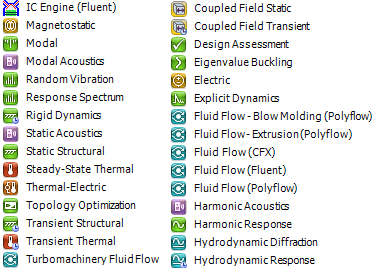
\includegraphics[height=6cm,width=1\textwidth,keepaspectratio]{cae_apps_ansys.png}
        \caption*{CAE apps in ANSYS}
        \label{fig:cae_apps_ansys.png}
    \end{subfigure}
    \begin{subfigure}{0.32\textwidth}
        \centering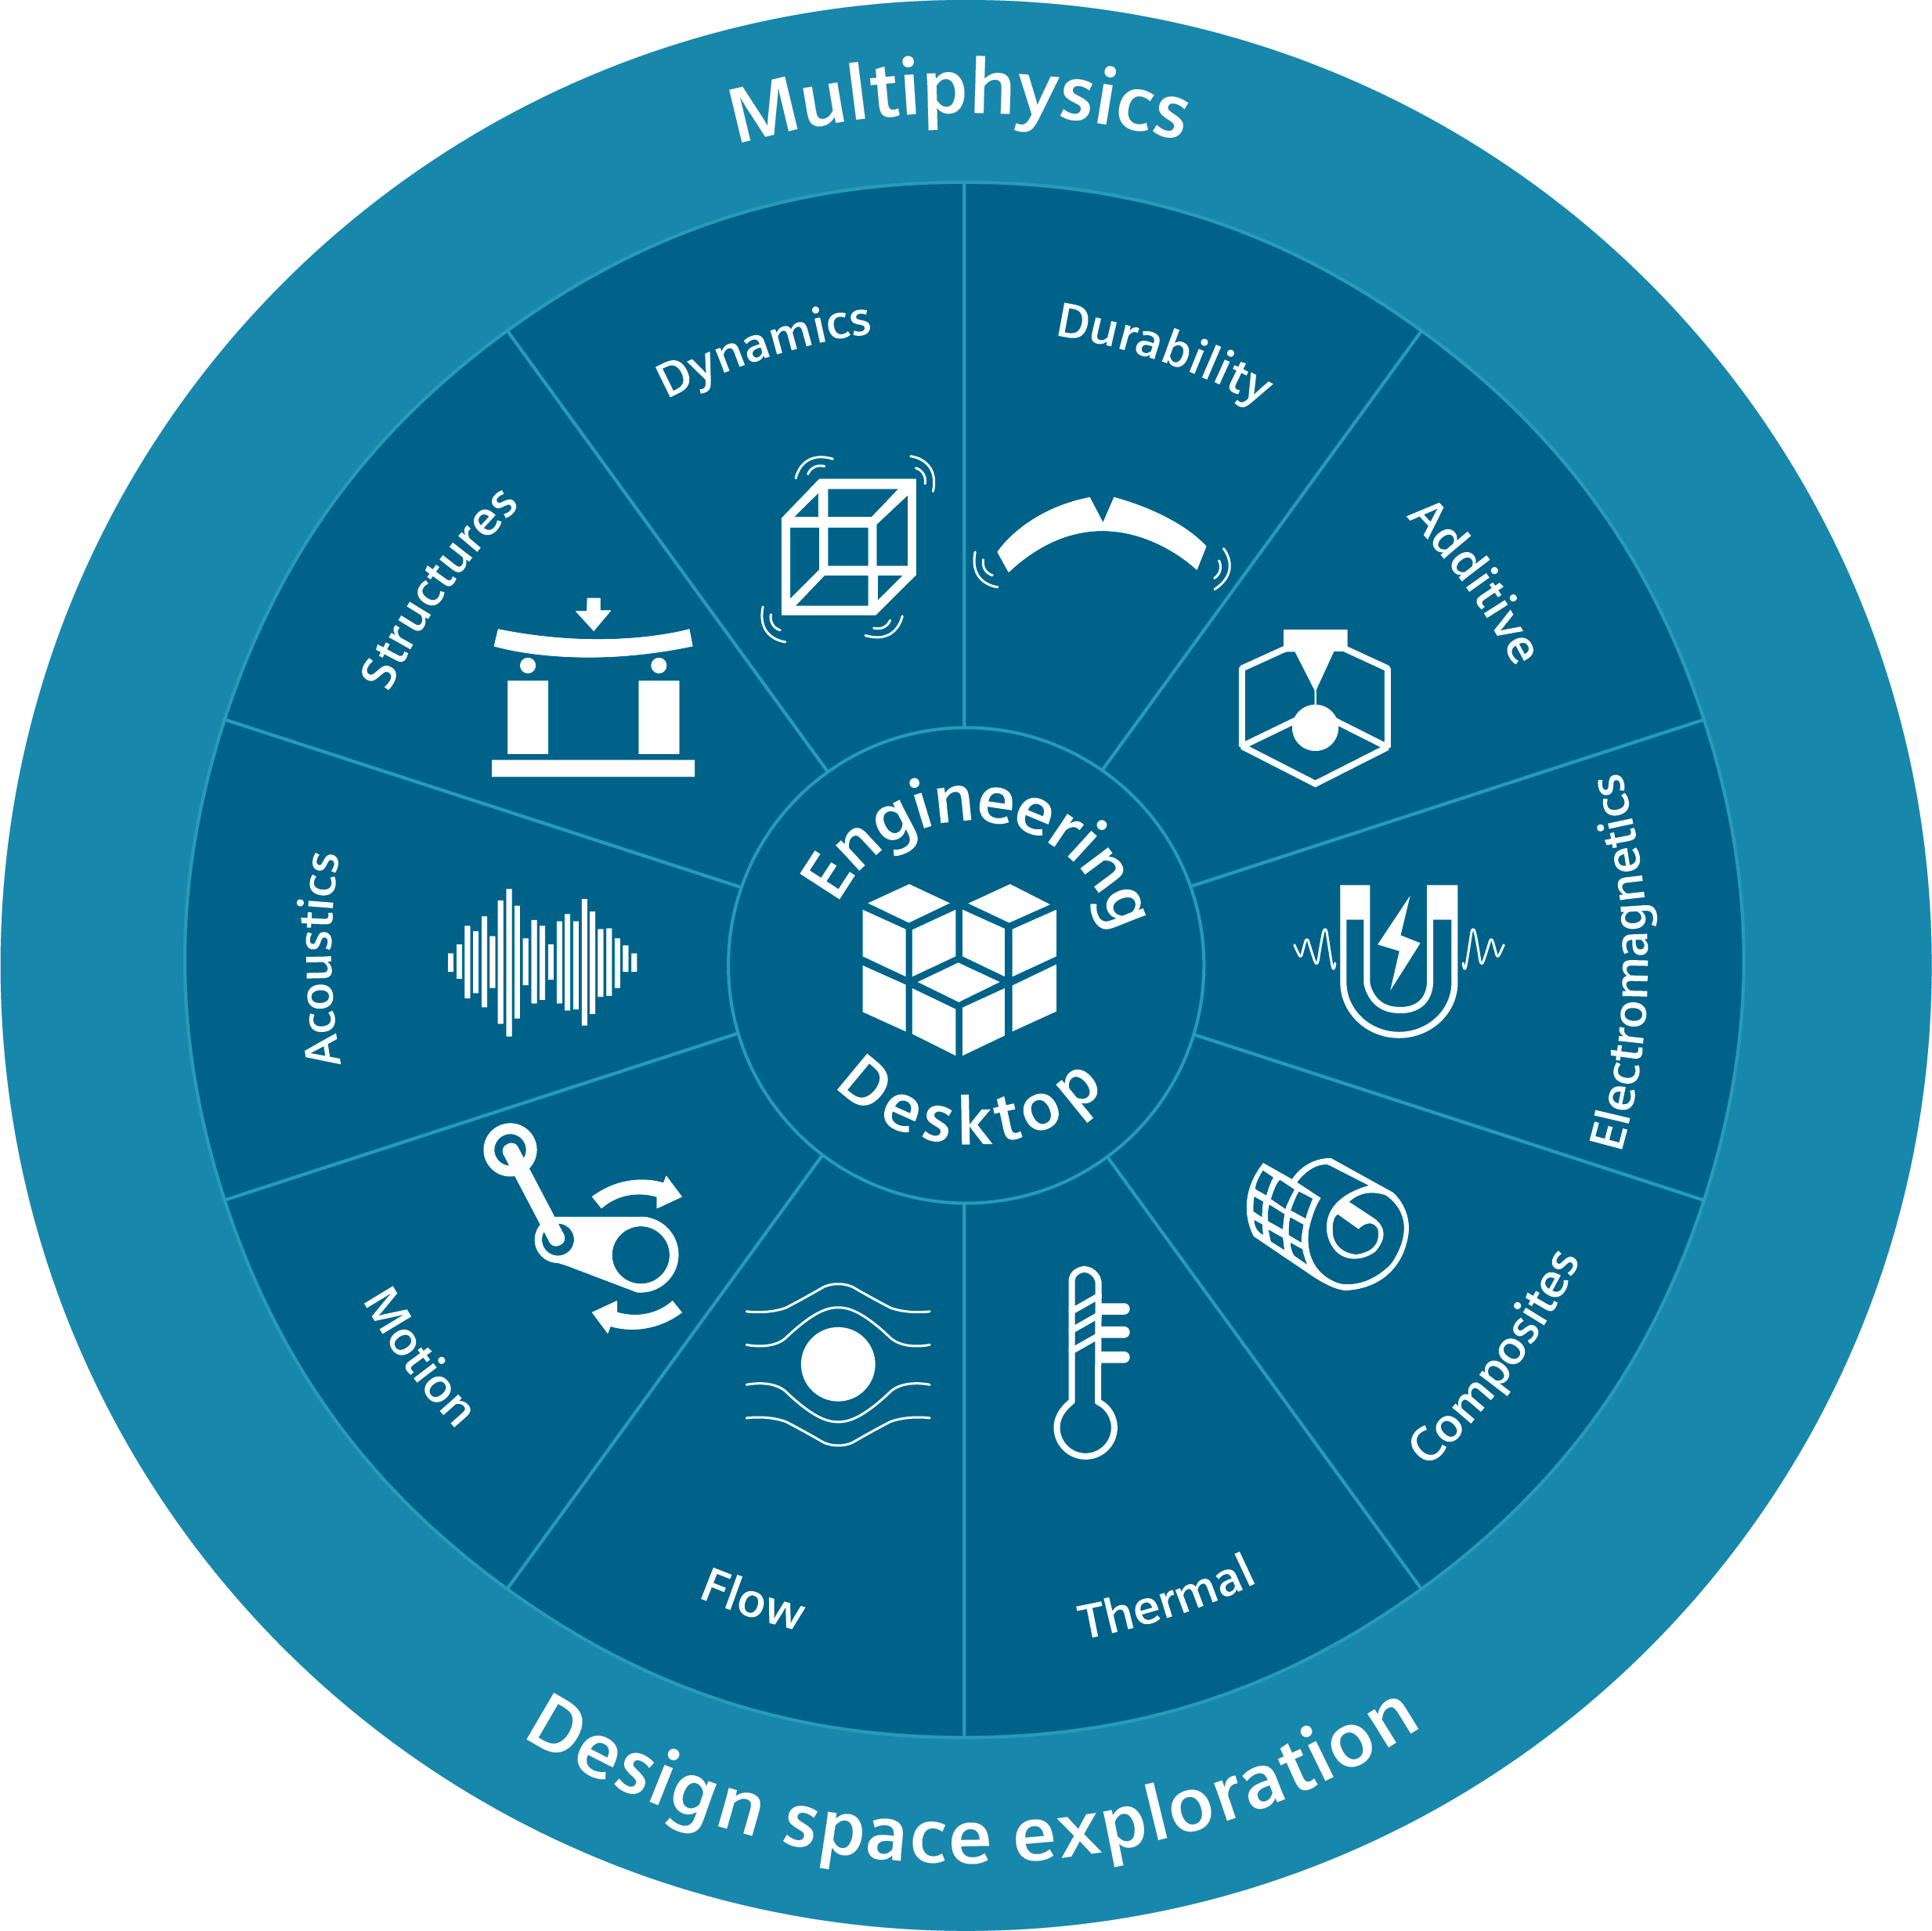
\includegraphics[height=6cm,width=1\textwidth,keepaspectratio]{cae_apps_nx.png}
        \caption*{CAE apps in Siemens NX}
        \label{fig:cae_apps_nx.png}
    \end{subfigure}
    \begin{subfigure}{0.32\textwidth}
        \centering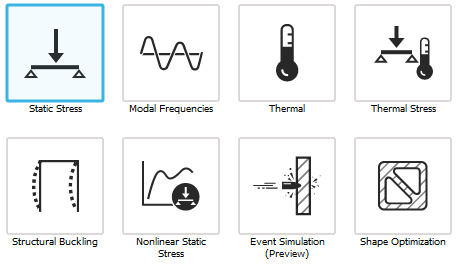
\includegraphics[height=6cm,width=1\textwidth,keepaspectratio]{cae_apps_fusion.png}
        \caption*{CAE apps in Fusion 360}
        \label{fig:cae_apps_fusion.png}
    \end{subfigure}
\end{figure}
\end{frame}

\begin{frame}[t]{Typical Engineering Tasks}
\framesubtitle{Static Stress}
\vspace{-0.3cm}
    \textbf{Goal}: Find \textit{deformation displacement} after applied required forces and torques.
    \begin{figure}[H]
        \begin{subfigure}{0.49\textwidth}
            \centering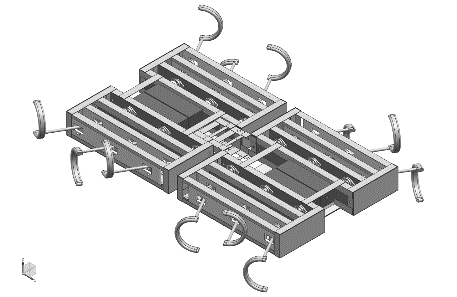
\includegraphics[height=5cm,width=1\textwidth,keepaspectratio]{cae_ex21.png}
            \label{fig:cae_ex21.png}
        \end{subfigure}
        \begin{subfigure}{0.49\textwidth}
            \centering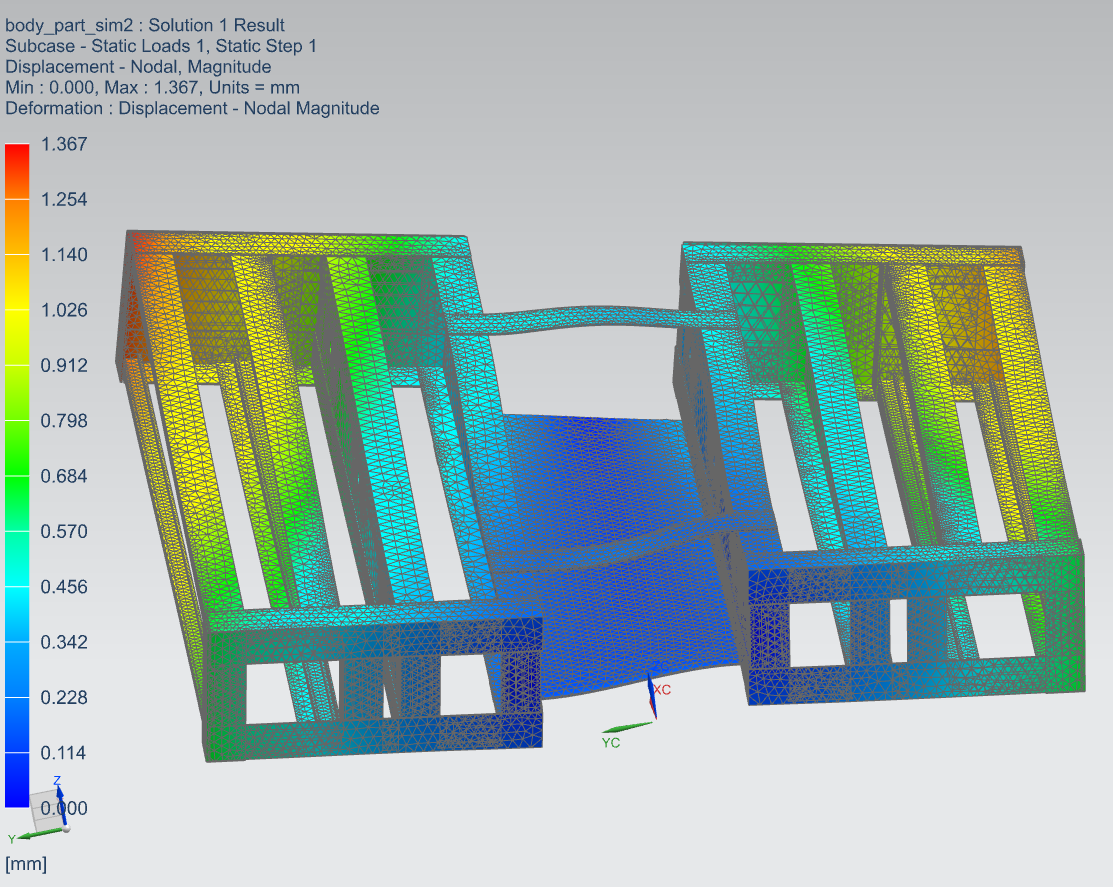
\includegraphics[height=5cm,width=1\textwidth,keepaspectratio]{cae_ex22.png}
            \label{fig:cae_ex22.png}
        \end{subfigure}
    \end{figure}
\end{frame}

\begin{frame}[t]{Typical Engineering Tasks}
    \framesubtitle{Rigid Dynamics}
    \vspace{-0.3cm}
    \textbf{Goal}: Find \textit{max motor torque} when the robot with needed dimensions and weight are moving though expected terrain.
    \begin{figure}[H]
        \href{https://gifyu.com/image/S7Hm8}{
            \centering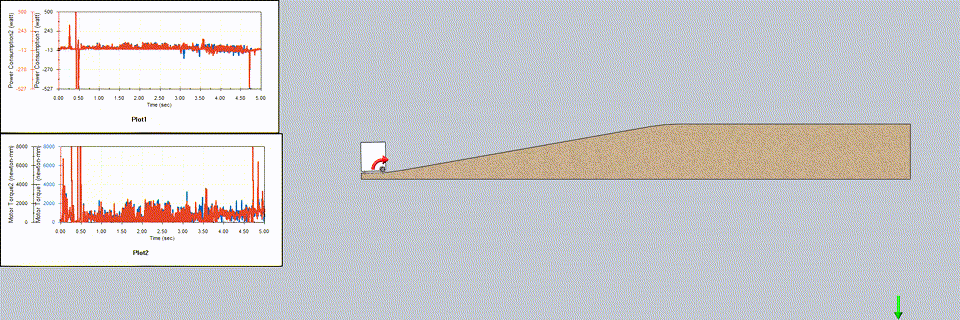
\includegraphics[height=5cm,width=1\textwidth,keepaspectratio]{cae_ex1_pic.png}}
        % \caption{Click on a picture for a video}
        \label{fig:cae_ex1_pic.png}
    \end{figure}
\end{frame}

\begin{frame}[t]{Typical Engineering Tasks}
    \framesubtitle{Motion Analysis}
    \vspace{-0.3cm}
    \textbf{Goal}: To understand the \textit{kinematics and dynamics} of designed robot in some situation.
    \begin{figure}[H]
        \href{https://gifyu.com/image/S7Hmr}{
            \centering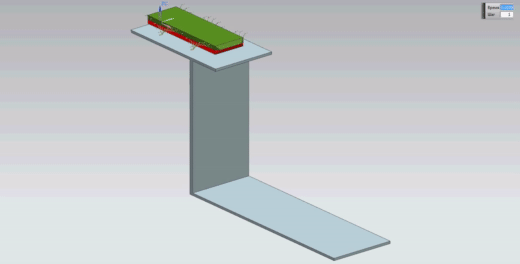
\includegraphics[height=5cm,width=1\textwidth,keepaspectratio]{cae_ex3_pic.png}}
        % \caption{Click on a picture for a video}
        \label{fig:cae_ex3_pic.png}
    \end{figure}
\end{frame}

\begin{frame}[t]{CAE General Workflow}
\framesubtitle{}
    \vspace{-0.6cm}
    \begin{figure}[H]
        \centering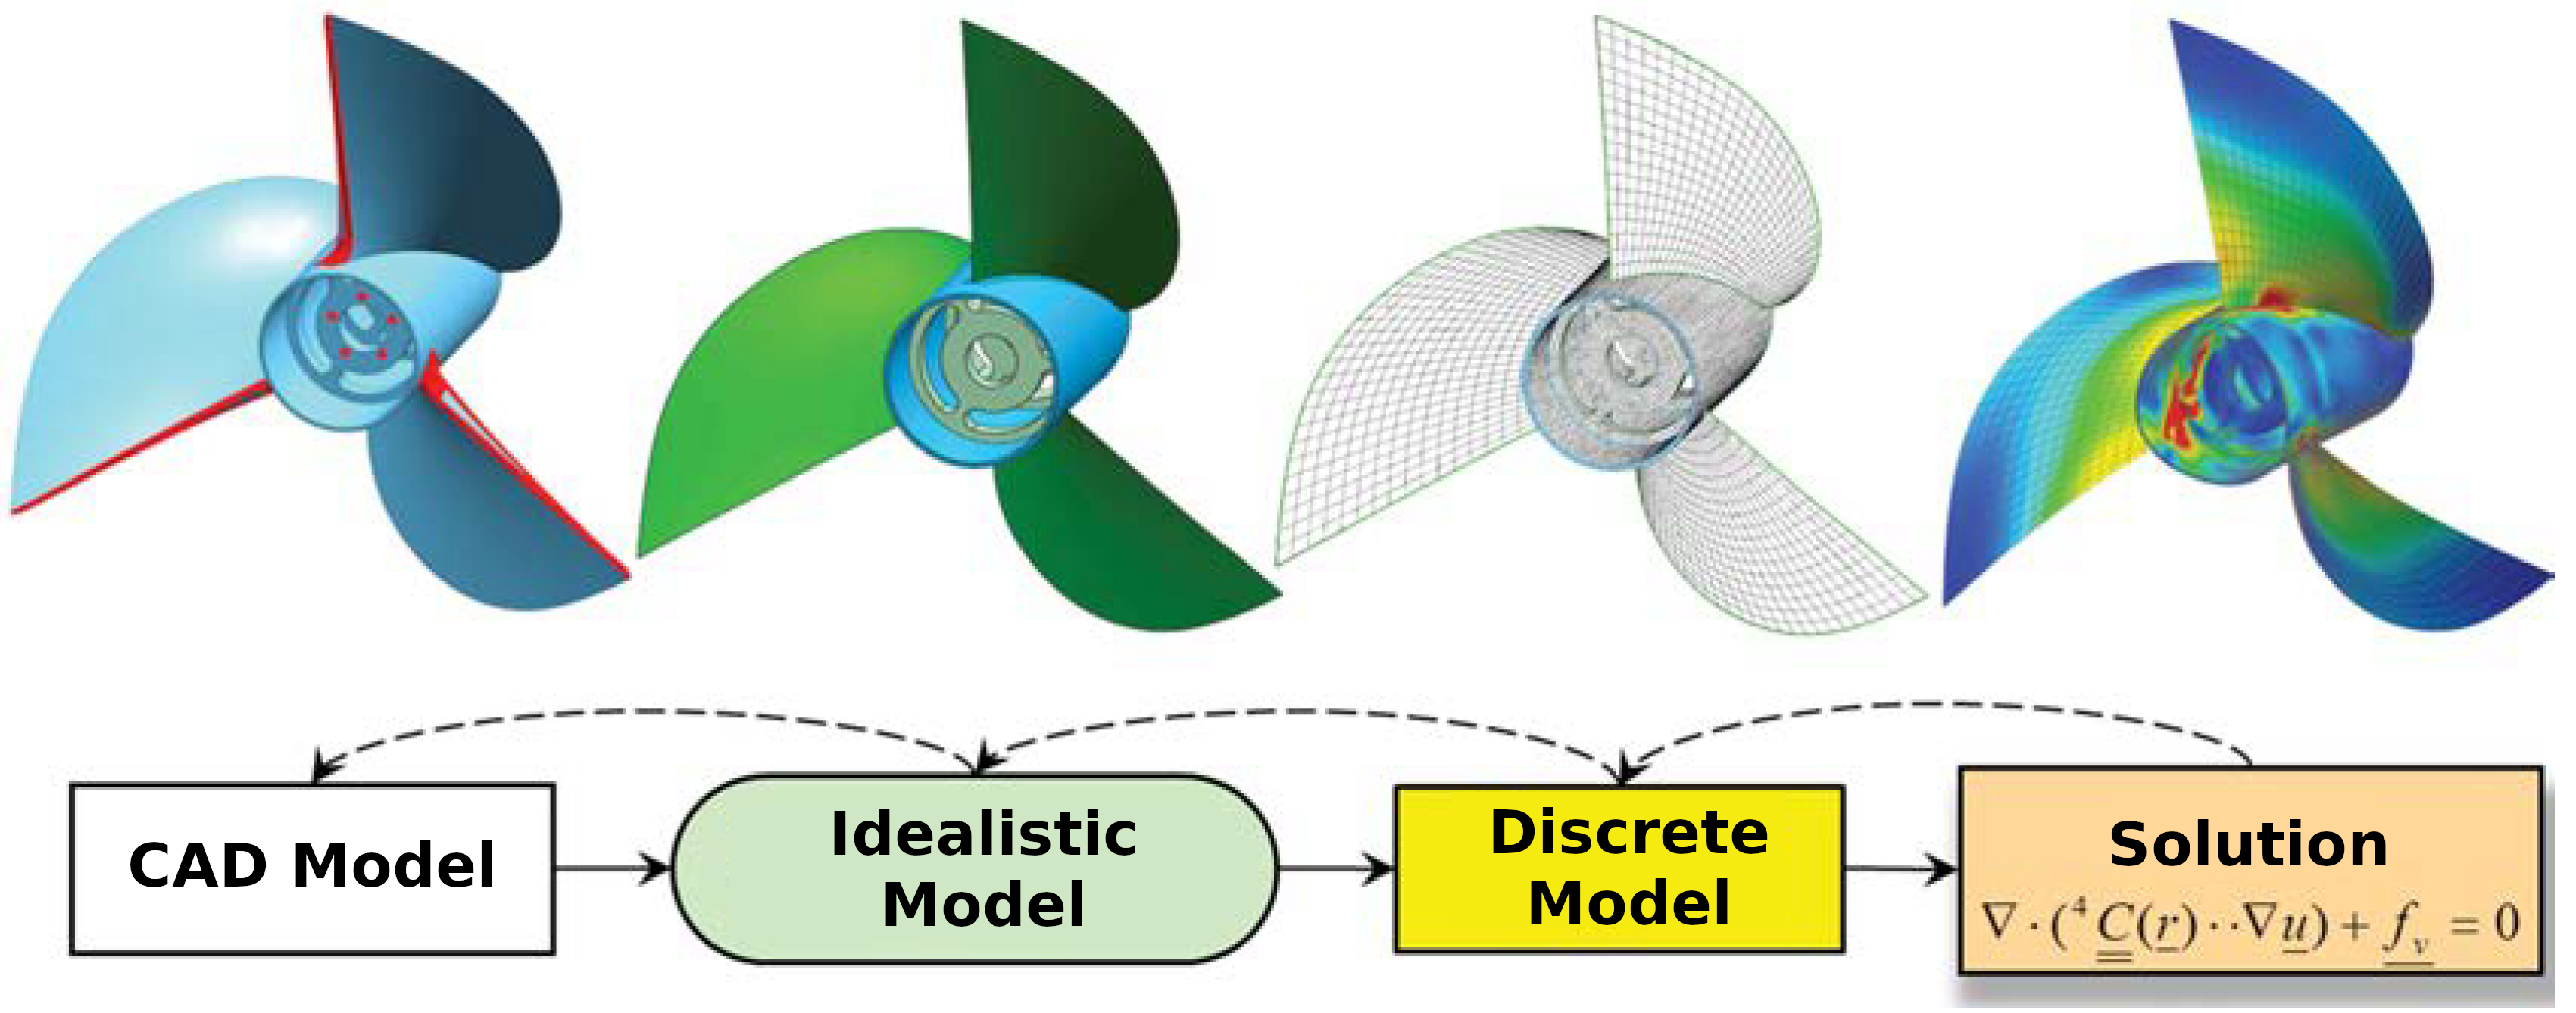
\includegraphics[height=6cm,width=1\textwidth,keepaspectratio]{cae_general_guideline.png}
        \label{fig:cae_general_guideline.png}
    \end{figure}
\end{frame}

\begin{frame}[t]{CAE Motion Workflow}
\framesubtitle{}
    \vspace{-0.6cm}
    \begin{figure}[H]
        \centering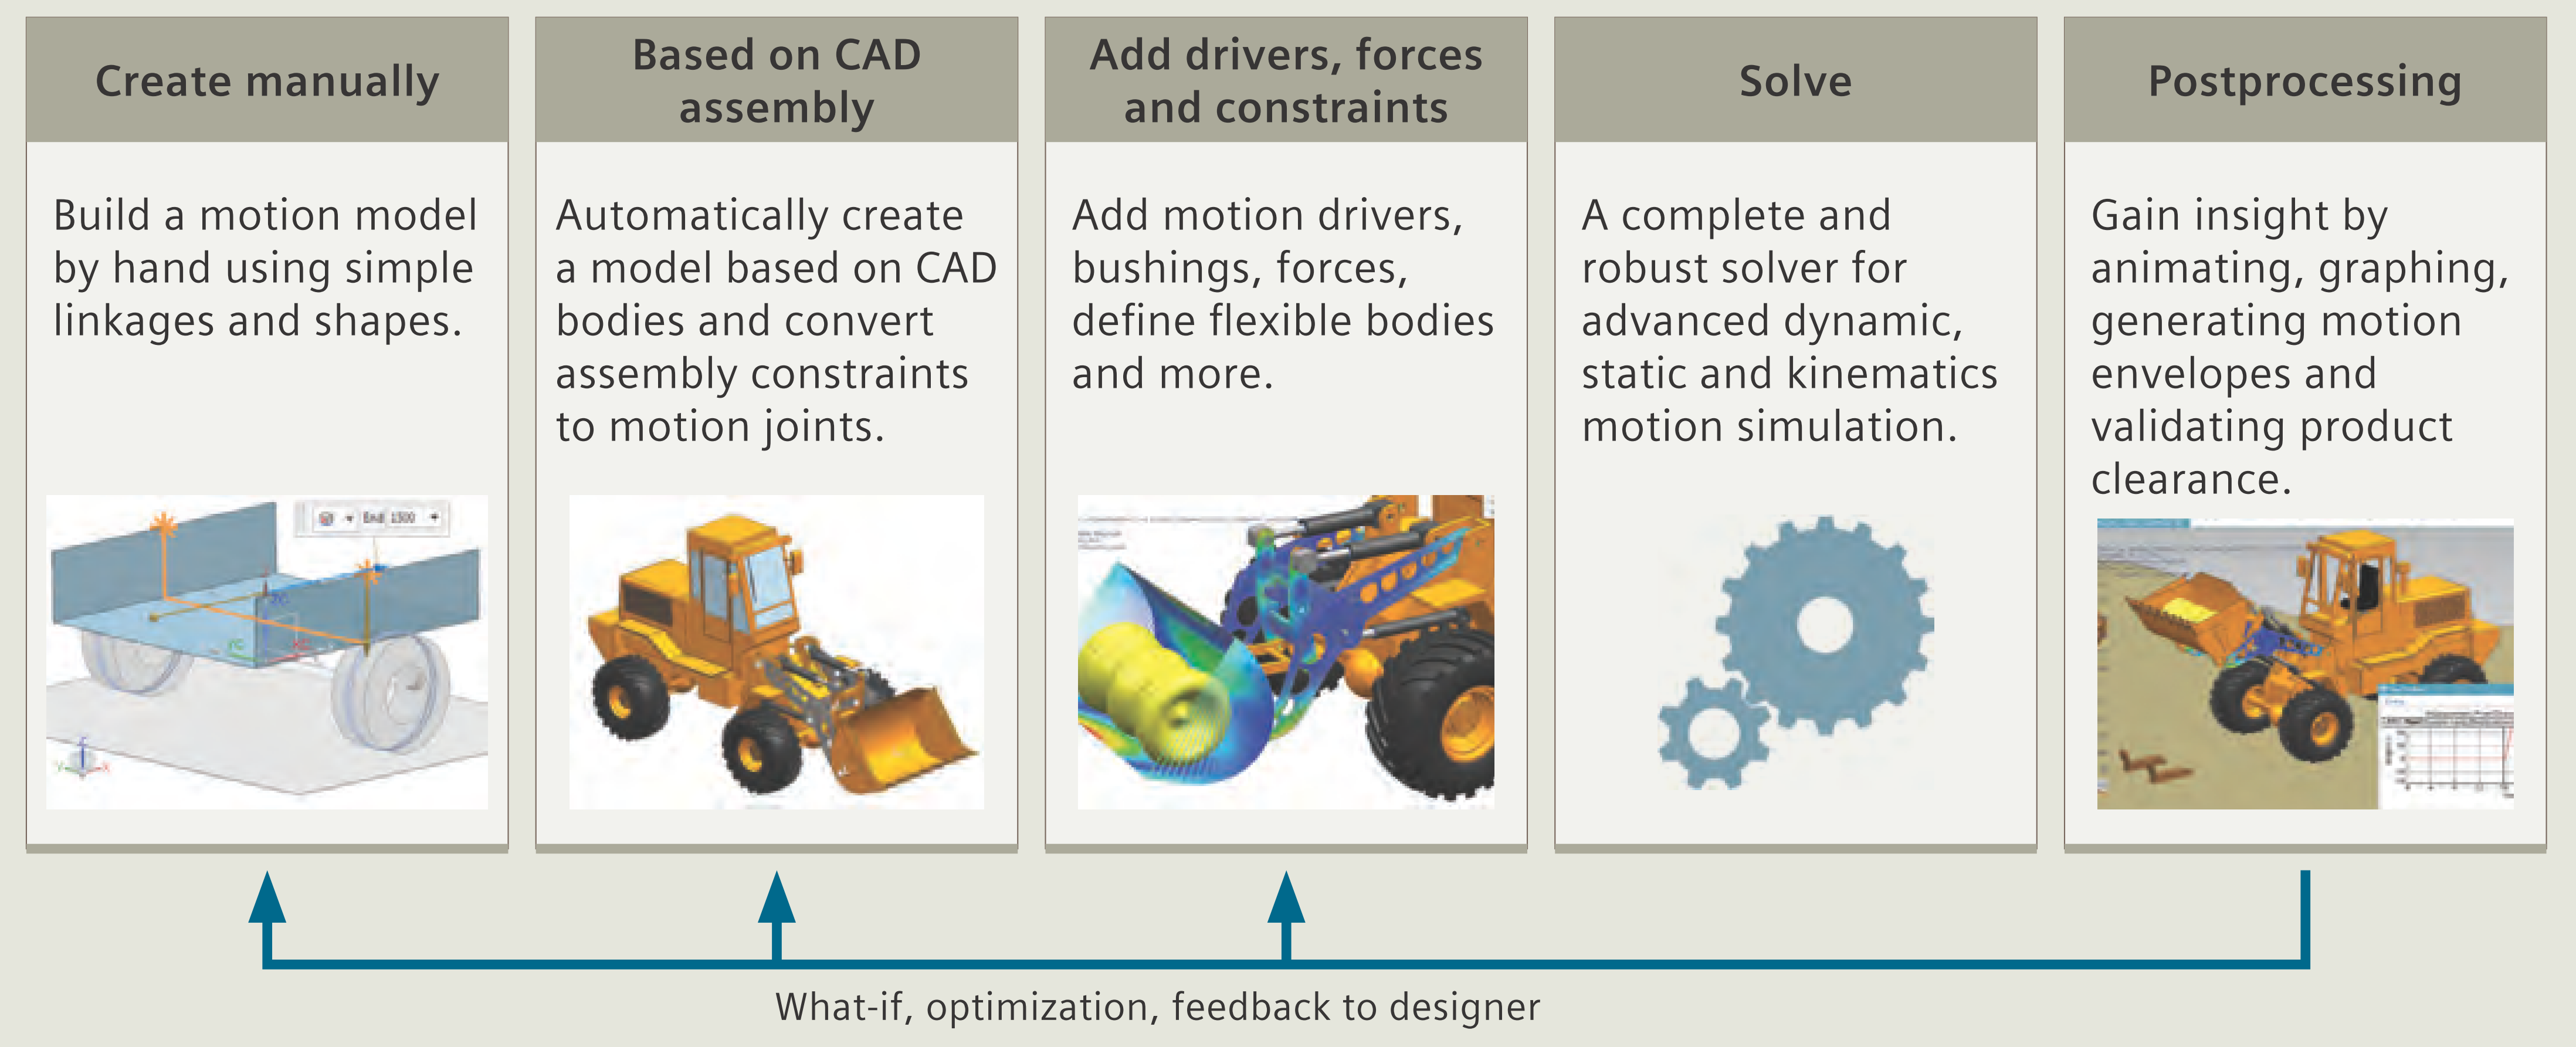
\includegraphics[height=6cm,width=1\textwidth,keepaspectratio]{cae_motion_guideline.png}
        \label{fig:file_name}
    \end{figure}
\end{frame}

\begin{frame}[t]{Solvers}
\framesubtitle{Definition}
Solver refers to a software tool that solves complex mathematical equations and models to simulate the behavior of physical systems.
\smallskip

The solver takes the \textbf{input data}, which includes the geometry of the system, the material properties, and boundary conditions, and then applies mathematical algorithms to calculate and solve the equations that describe the physical behavior of the system. The \textbf{output of the solver} is then used to evaluate the performance of the design and make necessary changes to improve it.
\smallskip

\textbf{Algorithm examples for Motion Analysis}: Euler-Lagrange, Newton-Euler, Kane's method
\smallskip

\textbf{Popular solvers}: NX Nastran (NX, Inventor, Fusion?), Abaqus (SolidWorks?), ANSYS (ANSYS)
\end{frame}

\begin{frame}[t]{Engineer's Guideline}
\framesubtitle{}
    \begin{enumerate}
        \item Formulate the task correctly (why and what we expect).
        \item Implement the idea with the help of CAE or other tools.
        \item Correctly interpret the obtained result.
        \item Propose a solution based on knowledge from <<3>>.
        \item Check the result.
    \end{enumerate}
\end{frame}

\begin{frame}[t]{Case Study}
\framesubtitle{Task formulation <<1>>}
    \begin{columns}[T,onlytextwidth]
        \begin{column}{0.49\textwidth}
            \textbf{General task}: Design the base for manipulator, which will not affects on the manipulator accuracy.
            \medskip

            \textbf{Reformulated task}: Check deformation displacement of the manipulator base.
        \end{column}
        \begin{column}{0.49\textwidth}
            \vspace{-0.6cm}
            \begin{figure}[H]
                \href{https://gifyu.com/image/S7HqU}{
                    \centering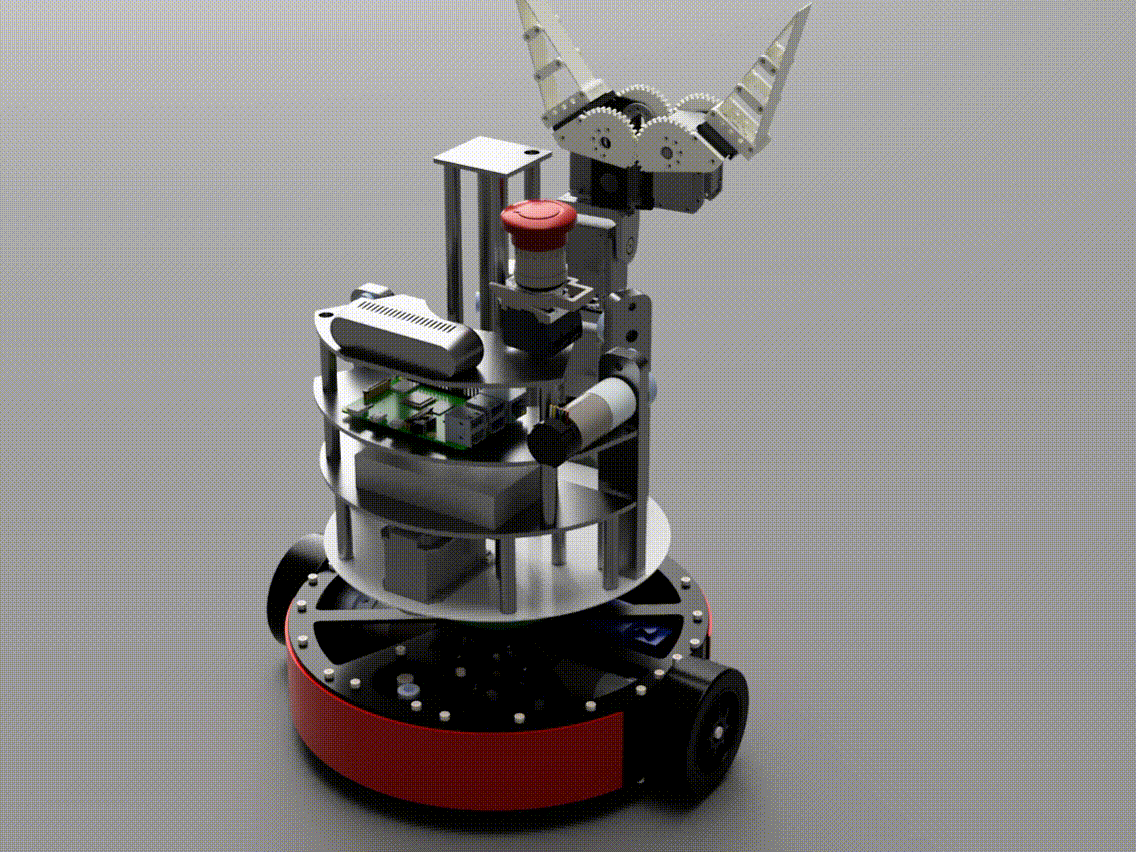
\includegraphics[height=6cm,width=1\textwidth,keepaspectratio]{eurobot_robot_pic.png}}
                \label{fig:eurobot_robot_pic.png}
            \end{figure}
        \end{column}
    \end{columns}
\end{frame}



\begin{frame}[t]{Case Study}
\framesubtitle{Implement and Interpret the result <<2-3>>}
    \vspace{-0.6cm}
    \begin{figure}[H]
        \centering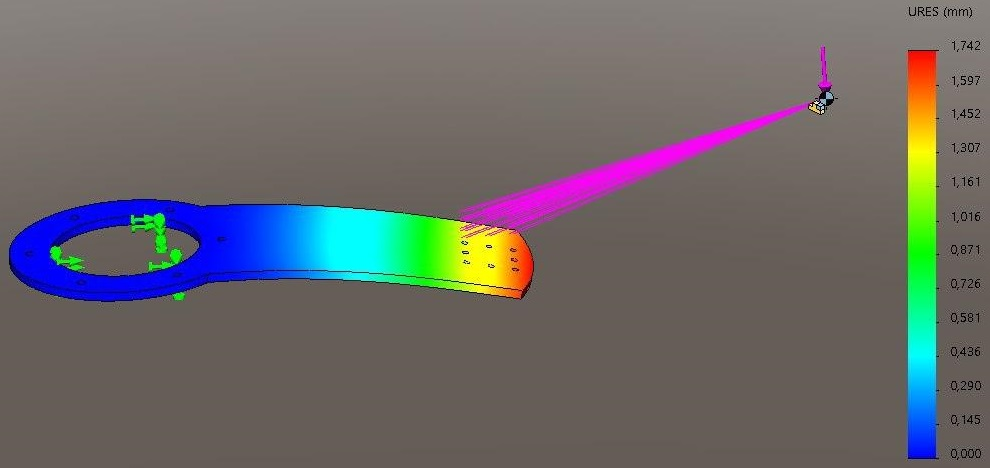
\includegraphics[height=6cm,width=1\textwidth,keepaspectratio]{cae_ex4.jpg}
        \label{fig:cae_ex4.jpg}
    \end{figure}
\end{frame}

\begin{frame}[t]{Case Study}
    \framesubtitle{Propose the solution <<4>>}
        \vspace{-0.6cm}
        \begin{figure}[H]
            \centering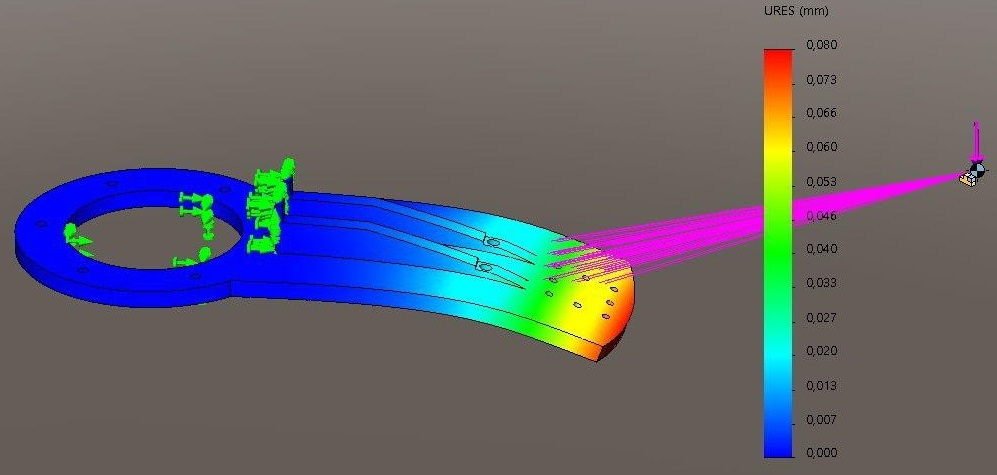
\includegraphics[height=6cm,width=1\textwidth,keepaspectratio]{cae_ex4_sol.jpg}
            \label{fig:cae_ex4_sol.jpg}
        \end{figure}
    \end{frame}



\begin{frame}[t]{Measure, Density, Interference}
    \framesubtitle{Video}
    \vspace{-0.6cm}
    \begin{figure}[H]
        \href{https://disk.yandex.ru/i/bYO6blkIitLJnQ}{
            \centering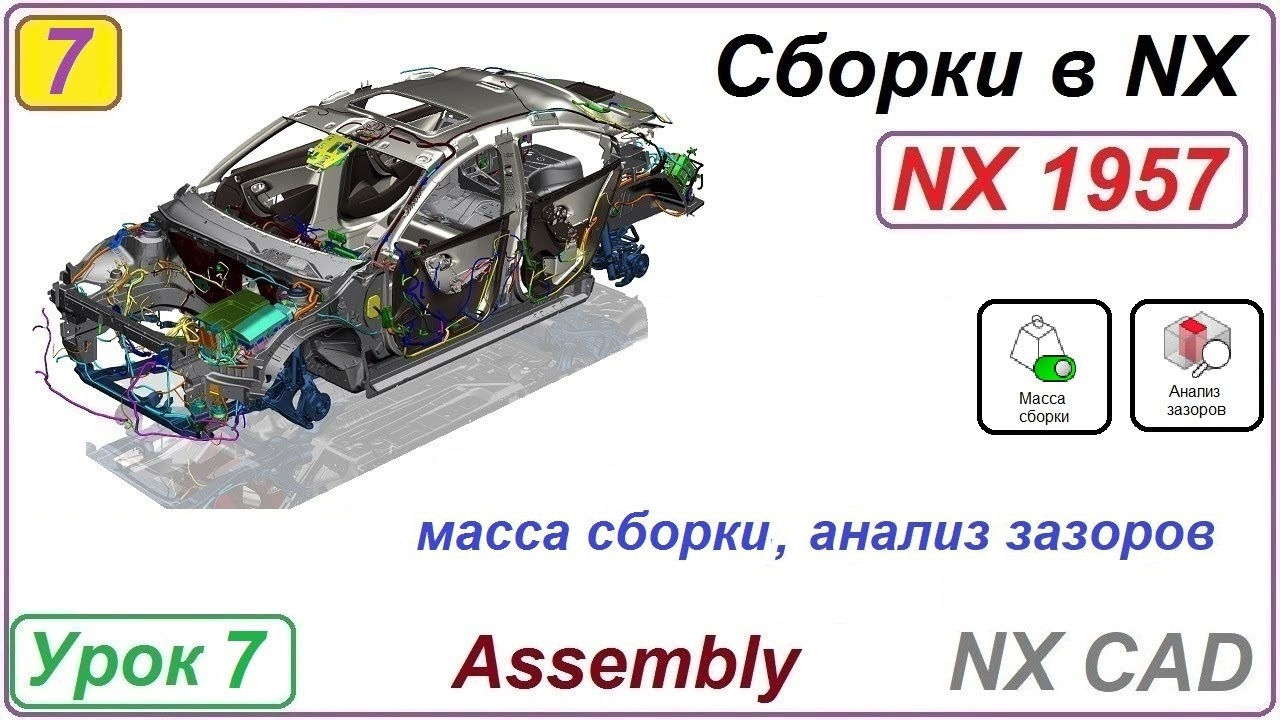
\includegraphics[height=6cm,width=1\textwidth,keepaspectratio]{mass_density_inteference_preview.jpg}}
        \label{fig:mass_density_inteference_preview.jpg}
    \end{figure}
\end{frame}

\begin{frame}[t]{Motion Analysis Applications}
\framesubtitle{}
\vspace{-0.8cm}
    \begin{columns}[T,onlytextwidth]
        \begin{column}{0.32\textwidth}
            \begin{center}
                \textbf{Animation Designer}
            \end{center}
            \vspace{-0.3cm}
            \begin{itemize}
                \footnotesize
                \item Can solve only kinematics.
                \item Can animate sketches
                \item You can draw some simple plots
                \item Can add collisions
            \end{itemize}
        \end{column}
        \begin{column}{0.32\textwidth}
            \begin{center}
                \textbf{Motion Analysis}
            \end{center}
            \vspace{-0.3cm}
            \begin{itemize}
                \footnotesize
                \item Can solve complex rigid/flexible multibody dynamics, statics and kinematics with high accuracy.
                \item CAD and analytical collisions
                \item Can simulate bearings, springs gears and etc.
                \item Friction model is quite accurate
            \end{itemize}
        \end{column}
        \begin{column}{0.32\textwidth}
            \begin{center}
                \textbf{Mechatronics Concept Designer}
            \end{center}
            \vspace{-0.3cm}
            \begin{itemize}
                \footnotesize
                \item Can solve dynamics and kinematics with low accuracy.
                \item System-level Design: it allows you to design and model complex mechatronic systems at a system-level, considering the interactions between mechanical, electrical, and software components.
                \item Can add a complex sequence of control operations
            \end{itemize}
        \end{column}
    \end{columns}
\end{frame}

\begin{frame}[t]{Motion Analysis Applications}
\framesubtitle{Summary}
\Large
\begin{center}
    If I want to check my concept on kinematics part, without designing a mechanism --- \textbf{Animation Designer}. \medskip

    If I want to deeply simulate my mechanism, find all forces, reaction forces, torques etc --- \textbf{Motion Analysis}. \medskip
    
    If I want to simulate a whole robot with some control stuff or whole convenor --- \textbf{Mechatronics Concept Designer}. 
\end{center}
\end{frame}

\begin{frame}[t]{Task 1}
\framesubtitle{}
\footnotesize
    The shown pendulum consists of a 4.54 $kg$ solid ball and 1.81 $kg$ solid rod.

    If it released from rest, when the $\theta = 0^\circ$, \textbf{determine the angle of rebound} after the ball strikes the wall and the pendulum swings up to the point of momentary rest. Take the restitution factor $e=0.6$ between the ball and the wall.
    \smallskip

    \alert{Answer}: $\theta_2 = 39.8^\circ$

    \begin{columns}[T,onlytextwidth]
        \begin{column}{0.49\textwidth}
            \begin{enumerate}
                \footnotesize
                \item Make a CAD model of the mechanism (or take it from \href{https://github.com/Lupasic/MaM_Inno_2023/tree/main/labs/CAE_DYN1/task_data/pendulum.zip}{\textit{labs/CAE\_DYN1/task\_data/pendulum.zip}})
                \item Assign the mass of the objects (have a mass and volume $\rightarrow$ can find density $\rightarrow$ change the density of the detail)
                \item Determine links, joints, collisions
                \item Configure a solver and solve the task
                \item Interpret the answer
            \end{enumerate}
        \end{column}
        \begin{column}{0.49\textwidth}
            \vspace{-1.2cm}

            \begin{figure}[H]
                \centering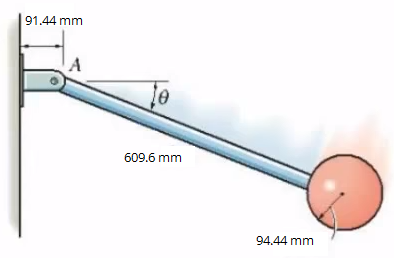
\includegraphics[height=4cm,width=1\textwidth,keepaspectratio]{task_1.png}
                \label{fig:task_1.png}
            \end{figure}
        \end{column}
    \end{columns}
\end{frame}

\begin{frame}[t]{Animation Designer}
\framesubtitle{Workflow}
    \vspace{-0.6cm}
    \begin{figure}[H]
        \centering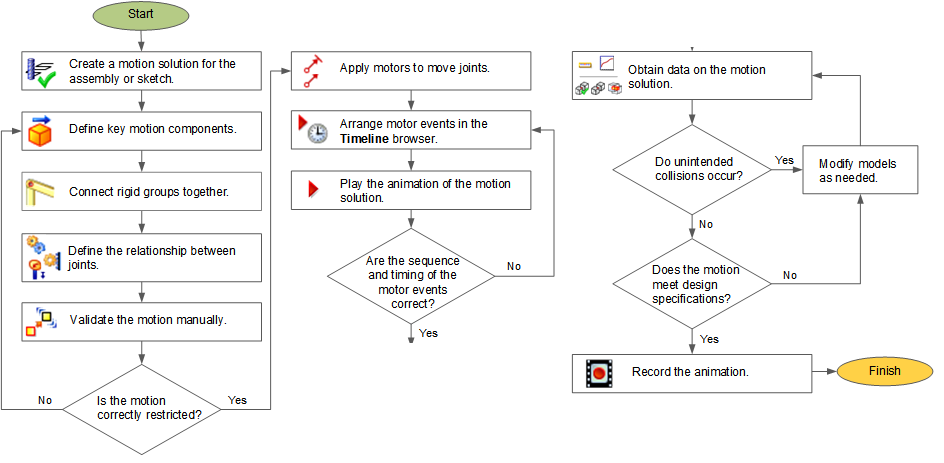
\includegraphics[height=6cm,width=1\textwidth,keepaspectratio]{motion_designer_workflow3.png}
        \label{fig:motion_designer_workflow3.png}
    \end{figure}
\end{frame}

\begin{frame}[t]{Animation Designer: Possibilites (1)}
    \framesubtitle{Video}
    \vspace{-0.6cm}
    \begin{figure}[H]
        \href{https://youtu.be/UKjR2YiDg2I}{
            \centering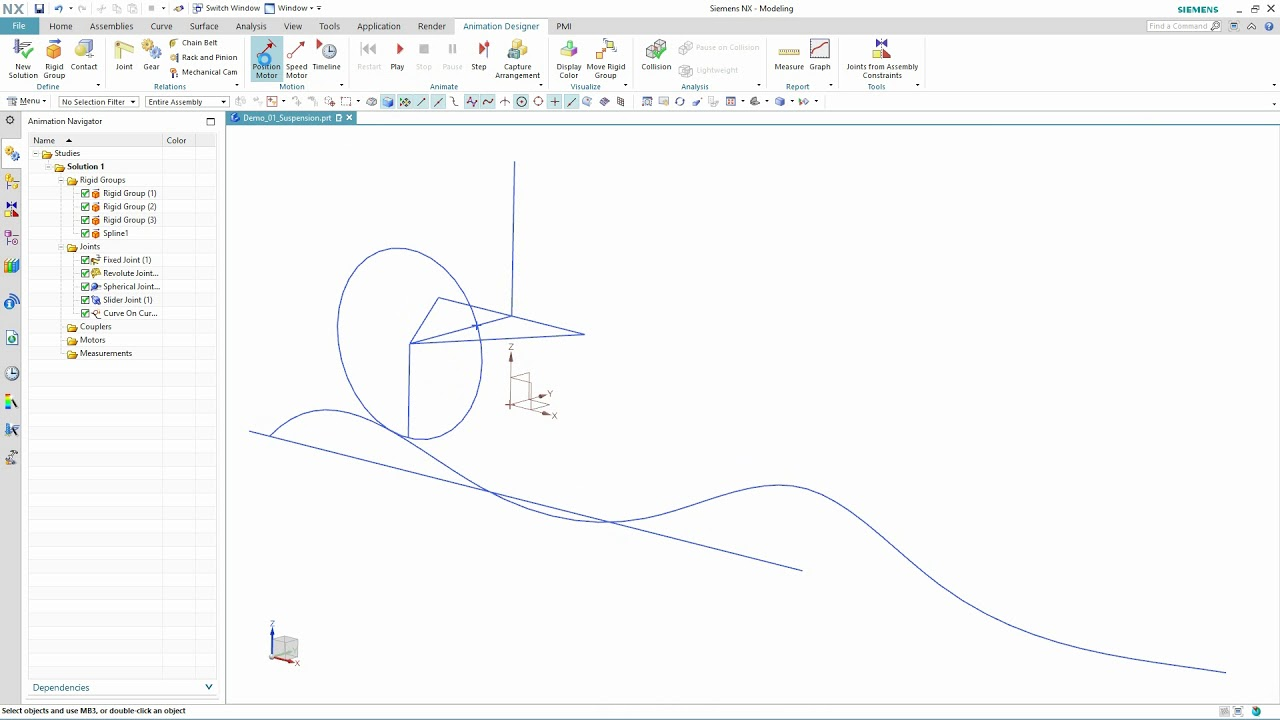
\includegraphics[height=6cm,width=1\textwidth,keepaspectratio]{anim_video1_preview.jpg}}
        % \caption{Click on a picture for a video}
        \label{fig:anim_video1_preview.jpg}
    \end{figure}
\end{frame}

\begin{frame}[t]{Animation Designer: Possibilites (2)}
    \framesubtitle{Video}
    \vspace{-0.6cm}
    \begin{figure}[H]
        \href{https://youtu.be/mlrptDMu42o}{
            \centering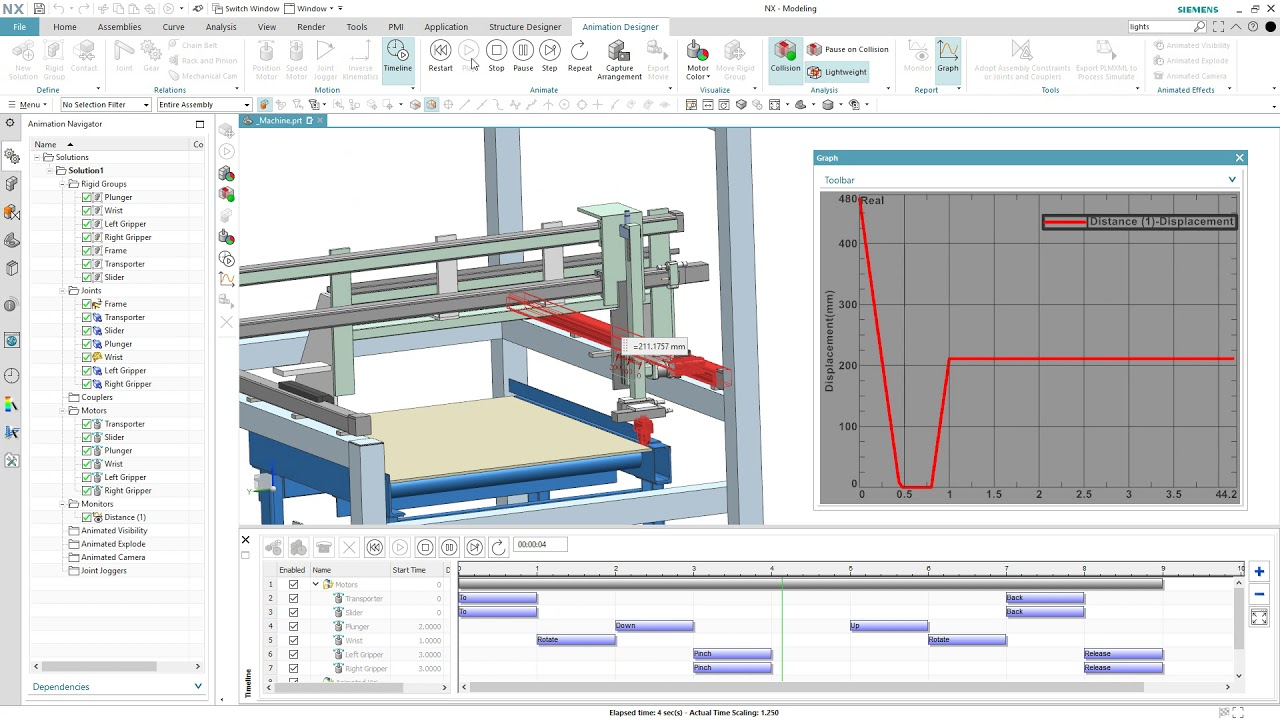
\includegraphics[height=6cm,width=1\textwidth,keepaspectratio]{anim_video2_preview.jpg}}
        % \caption{Click on a picture for a video}
        \label{fig:anim_video2_preview.jpg}
    \end{figure}
\end{frame}

\begin{frame}[t]{Animation Designer}
    \framesubtitle{Task 1}
    \vspace{-0.6cm}
    \begin{figure}[H]
        \href{https://disk.yandex.ru/i/Jn6CjUOzpJXqhg}{
            \centering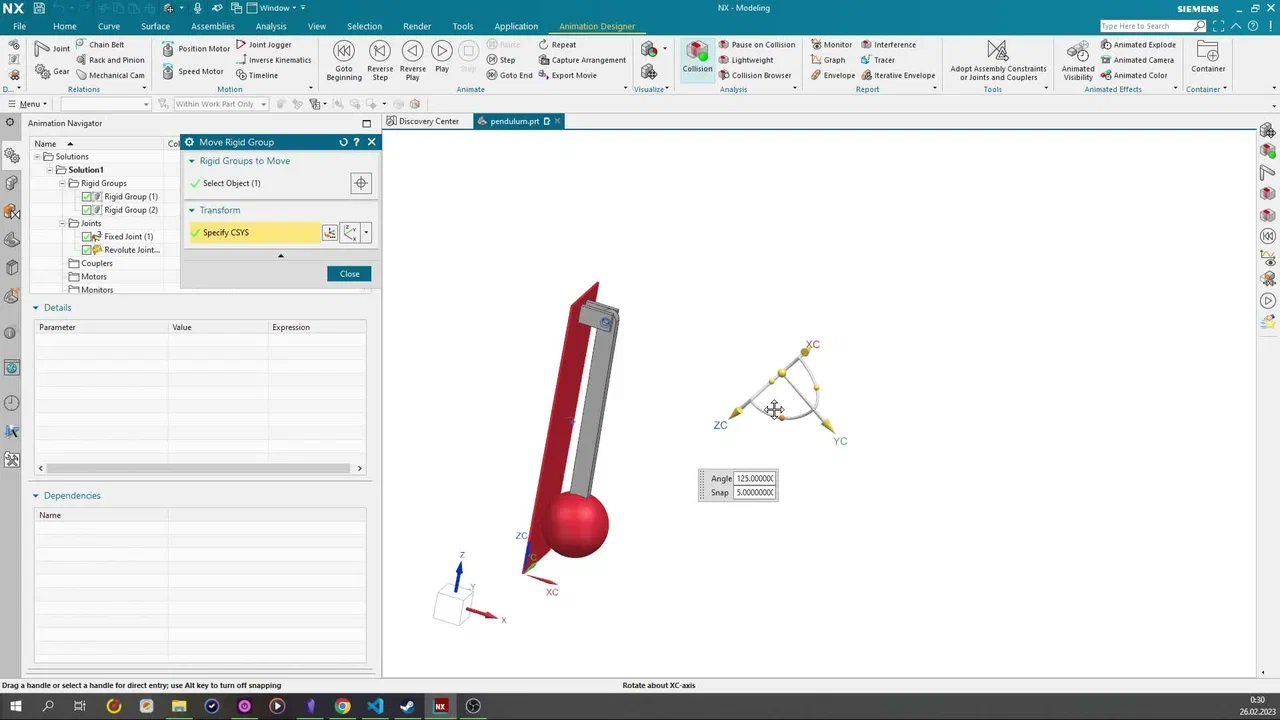
\includegraphics[height=6cm,width=1\textwidth,keepaspectratio]{anim_video_preview.png}}
        % \caption{Click on a picture for a video}
        \label{fig:anim_video_preview.png}
    \end{figure}
\end{frame}

\begin{frame}[t]{Mechatronics Concept Designer}
\framesubtitle{Global Workflow}
    \vspace{-0.6cm}
    \begin{figure}[H]
        \centering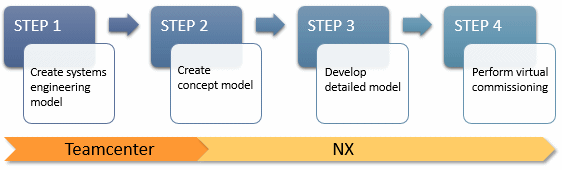
\includegraphics[height=6cm,width=1\textwidth,keepaspectratio]{mcd_overview_flowchart.png}
        \label{fig:mcd_overview_flowchart.png}
    \end{figure}
\end{frame}

\begin{frame}[t]{Mechatronics Concept Designer}
\framesubtitle{Concept Model}
    \vspace{-0.6cm}
    \begin{figure}[H]
        \centering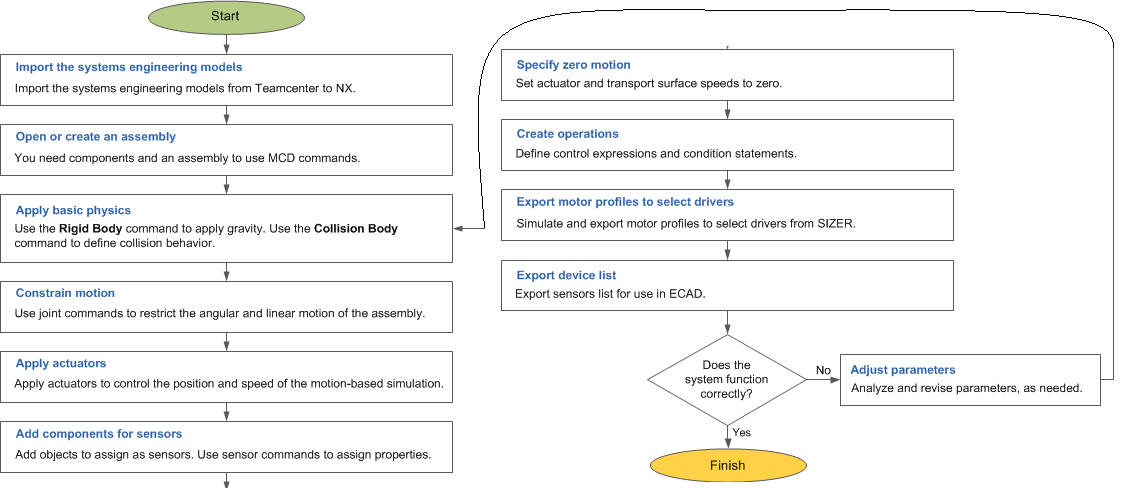
\includegraphics[height=6cm,width=1\textwidth,keepaspectratio]{mcd_concept_model_flowchart.png}
        \label{fig:mcd_concept_model_flowchart.png}
    \end{figure}
\end{frame}

\begin{frame}[t]{Mechatronics Concept Designer}
\framesubtitle{Detailed Model}
    \vspace{-0.6cm}
    \begin{figure}[H]
        \centering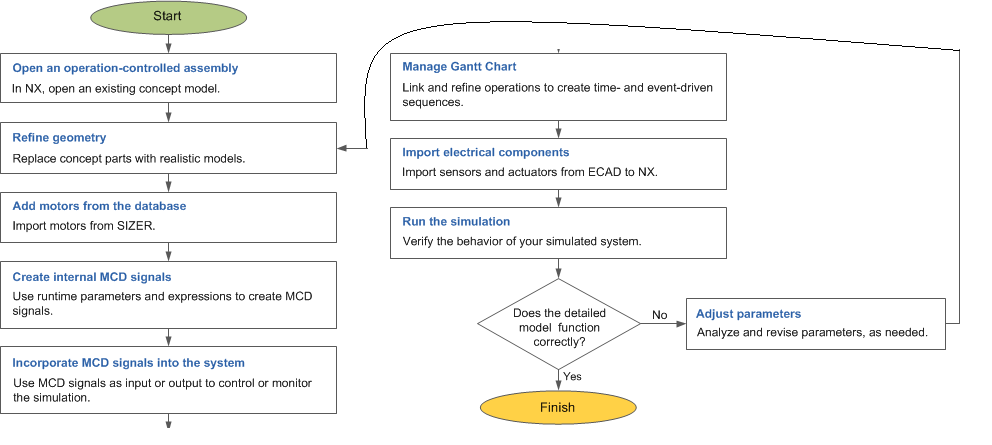
\includegraphics[height=6cm,width=1\textwidth,keepaspectratio]{mcd_detailed_model_flowchart.png}
        \label{fig:mcd_detailed_model_flowchart.png}
    \end{figure}
\end{frame}

\begin{frame}[t]{Mechatronics Concept Designer: Possibilites (1)}
    \framesubtitle{Video}
    \vspace{-0.6cm}
    \begin{figure}[H]
        \href{https://youtu.be/x3ncDZdelRY?t=2381}{
            \centering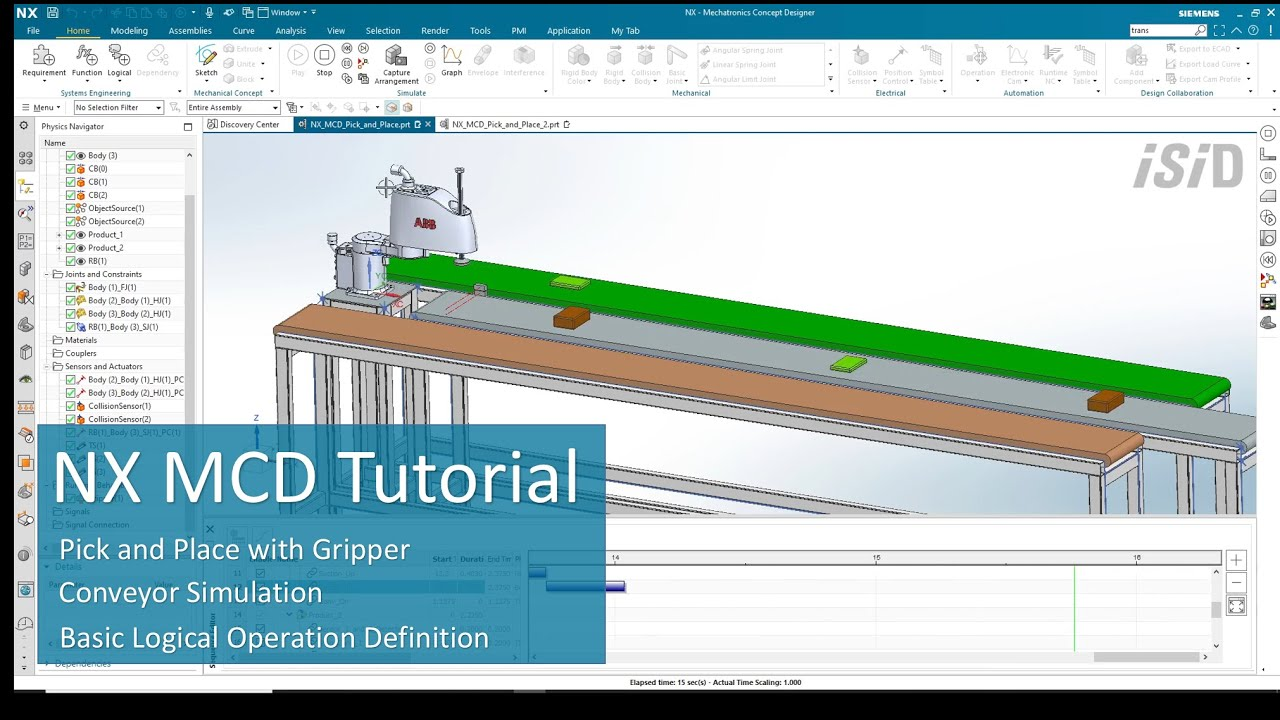
\includegraphics[height=6cm,width=1\textwidth,keepaspectratio]{mcd_video1_preview.jpg}}
        % \caption{Click on a picture for a video}
        \label{fig:mcd_video1_preview.jpg}
    \end{figure}
\end{frame}

\begin{frame}[t]{Mechatronics Concept Designer: Possibilites (2)}
    \framesubtitle{Video}
    \vspace{-0.6cm}
    \begin{figure}[H]
        \href{https://youtu.be/ZvrE2IfrfgI}{
            \centering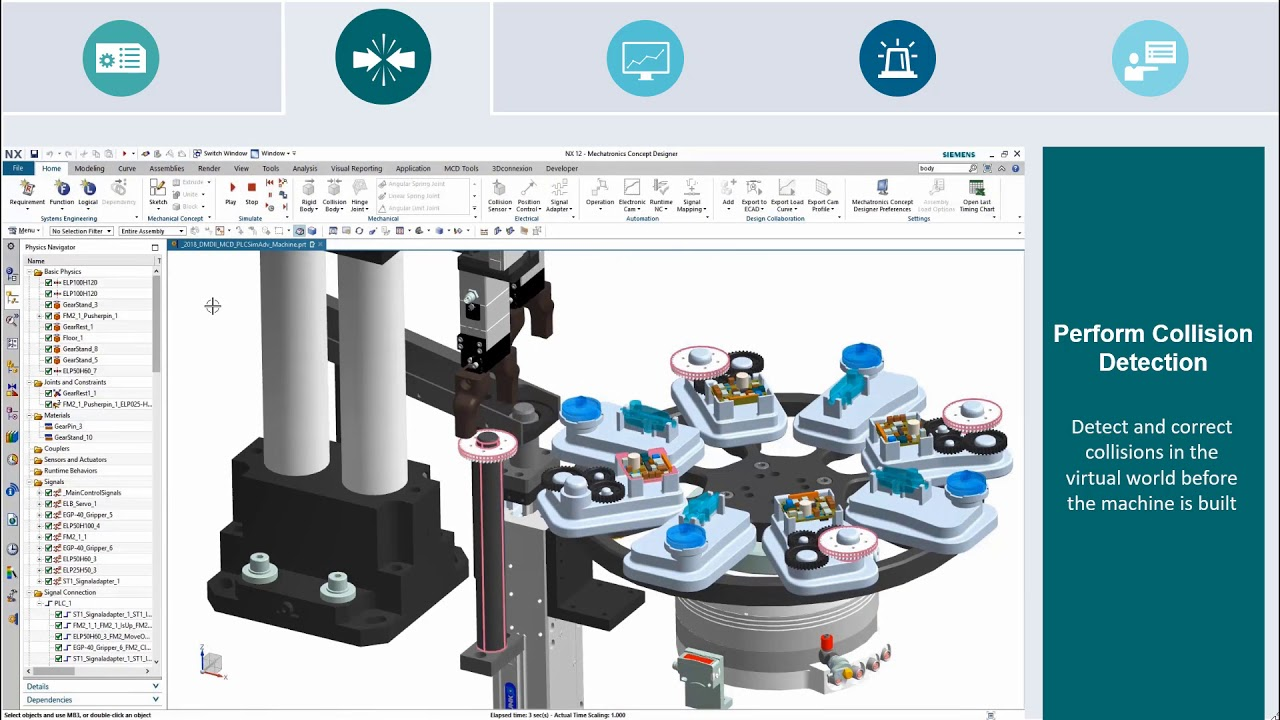
\includegraphics[height=6cm,width=1\textwidth,keepaspectratio]{mcd_video2_preview.jpg}}
        % \caption{Click on a picture for a video}
        \label{fig:mcd_video2_preview.jpg}
    \end{figure}
\end{frame}

\begin{frame}[t]{Mechatronics Concept Designer}
    \framesubtitle{Task 1}
    \vspace{-0.6cm}
    \begin{figure}[H]
        \href{https://disk.yandex.ru/i/F-FYIX3xmzNACg}{
            \centering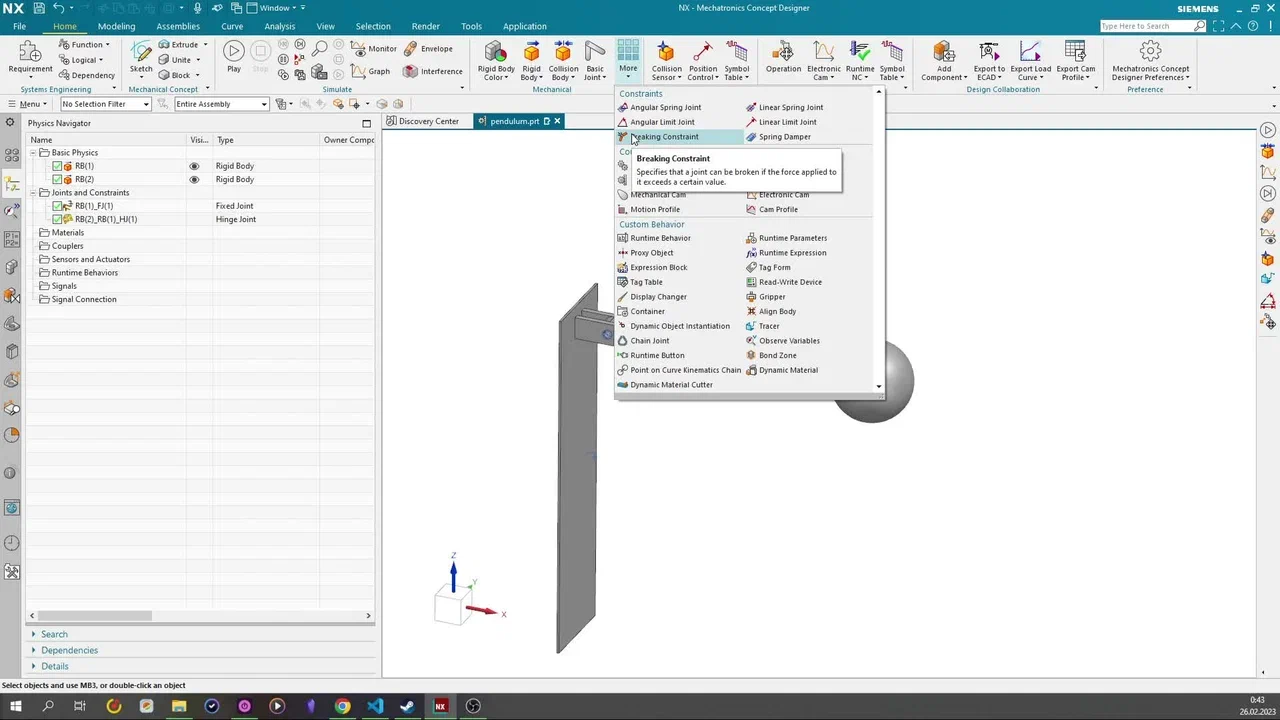
\includegraphics[height=6cm,width=1\textwidth,keepaspectratio]{mcd_video_preview.png}}
        % \caption{Click on a picture for a video}
        \label{fig:mcd_video_preview.png}
    \end{figure}
\end{frame}

\begin{frame}[t]{Motion Analysis: Workflow}
\framesubtitle{}
    \vspace{-0.6cm}
    \begin{figure}[H]
        \centering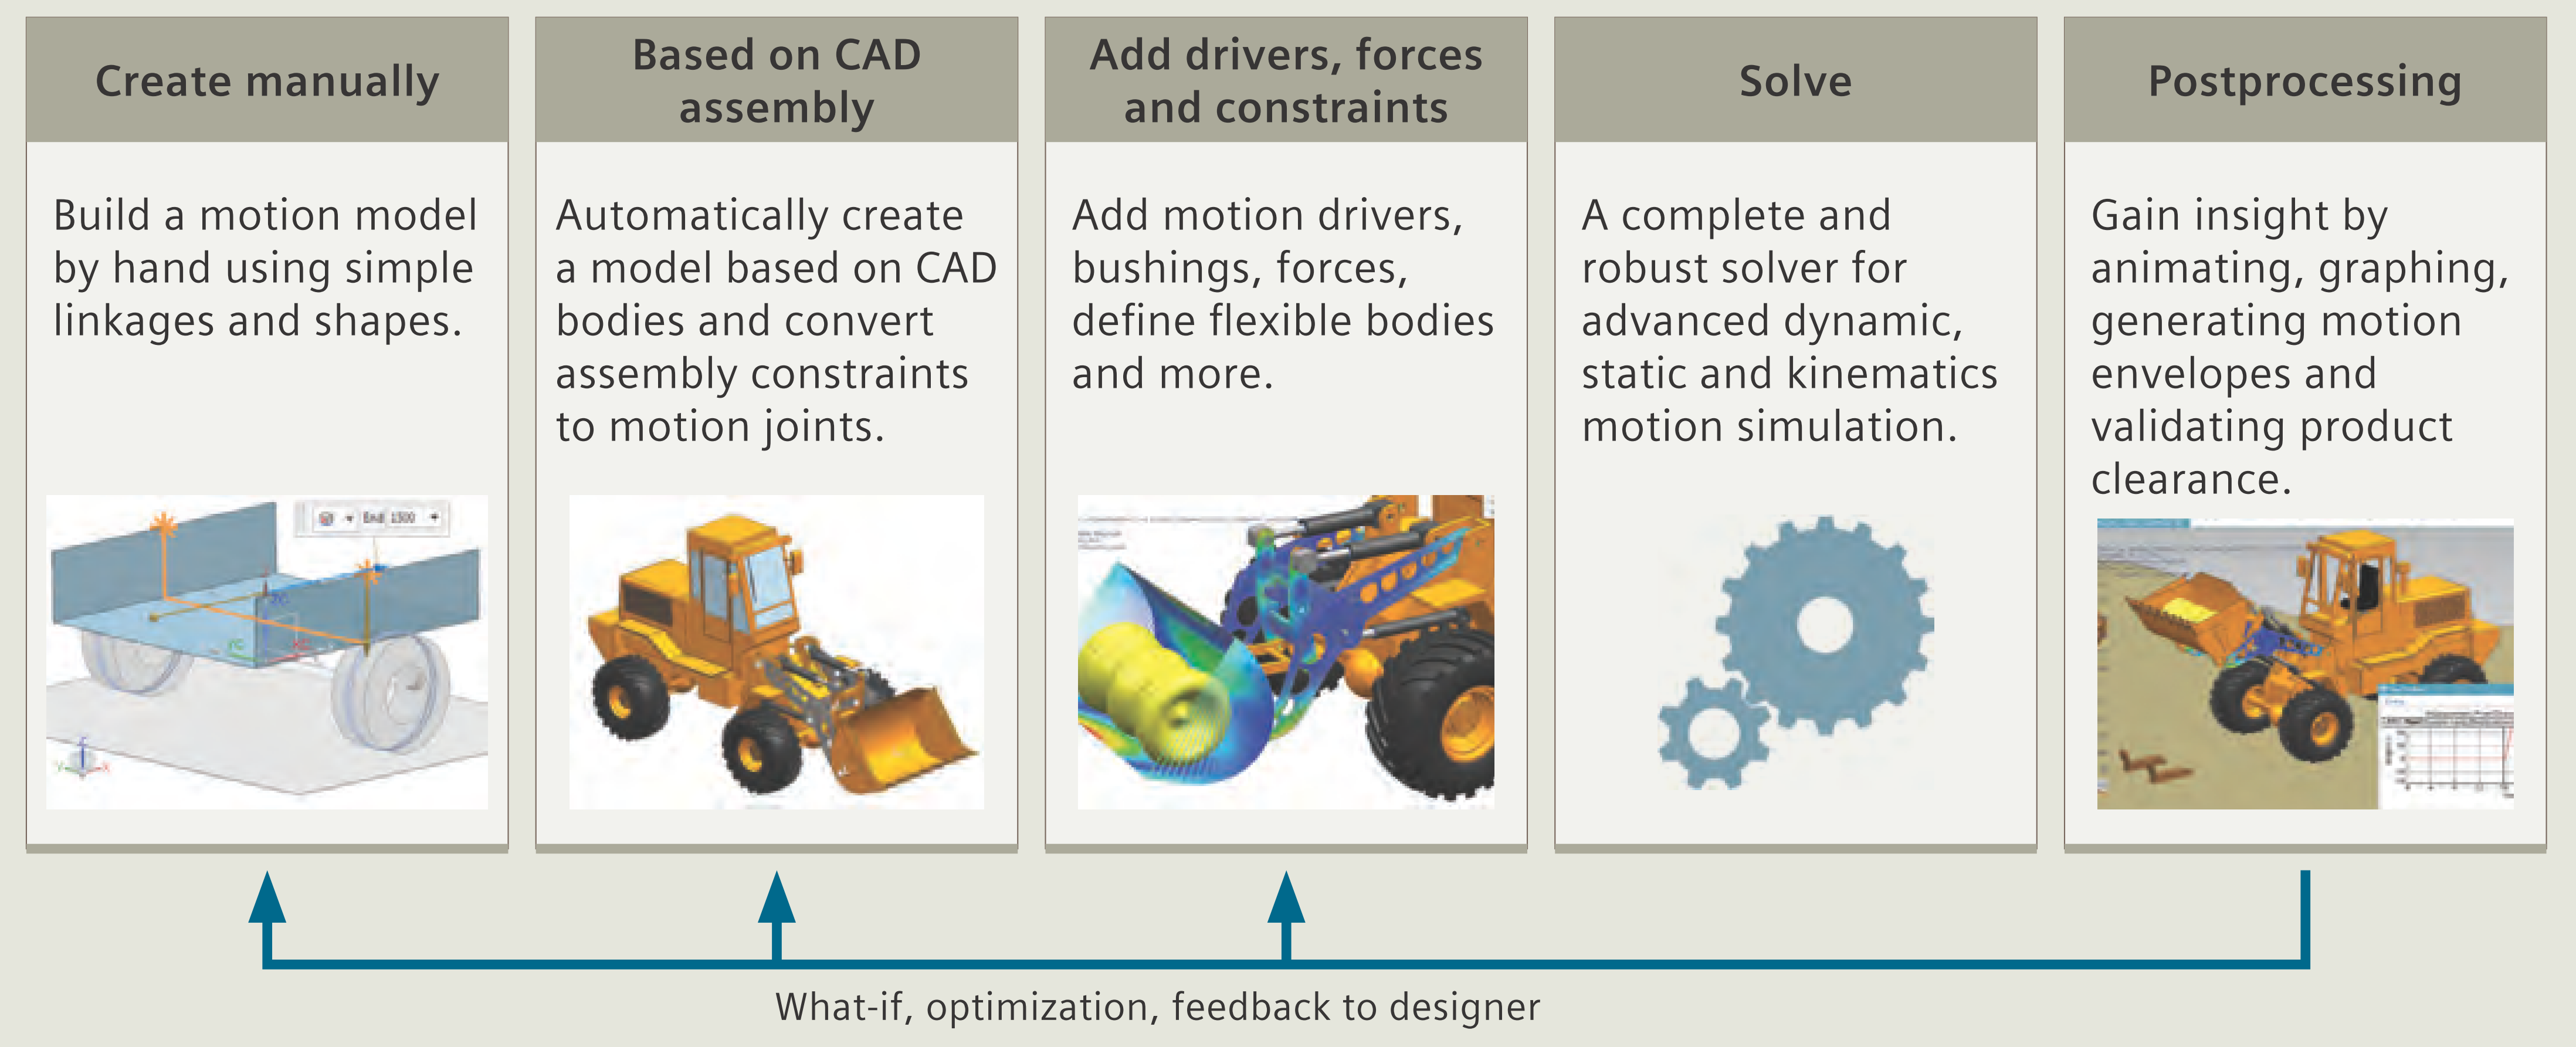
\includegraphics[height=6cm,width=1\textwidth,keepaspectratio]{cae_motion_guideline.png}
        \label{fig:cae_motion_guideline.png}
    \end{figure}
\end{frame}

\begin{frame}[t]{Motion Analysis: Possibilites (1)}
    \framesubtitle{Video}
    \vspace{-0.6cm}
    \begin{figure}[H]
        \href{https://www.youtube.com/watch?v=biMRRdMpJno}{
            \centering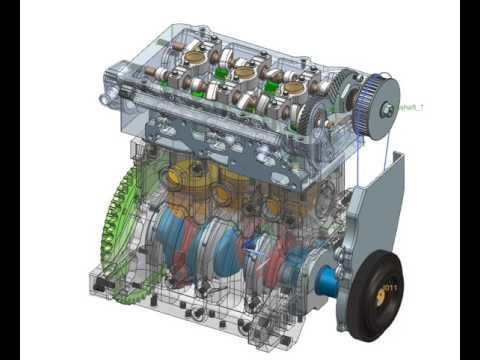
\includegraphics[height=6cm,width=1\textwidth,keepaspectratio]{motion_video1_preview.jpg}}
        % \caption{Click on a picture for a video}
        \label{fig:motion_video1_preview.jpg}
    \end{figure}
\end{frame}

\begin{frame}[t]{Motion Analysis: Possibilites (2)}
    \framesubtitle{Video}
    \vspace{-0.6cm}
    \begin{figure}[H]
        \href{https://youtu.be/p_bHL19dTRY}{
            \centering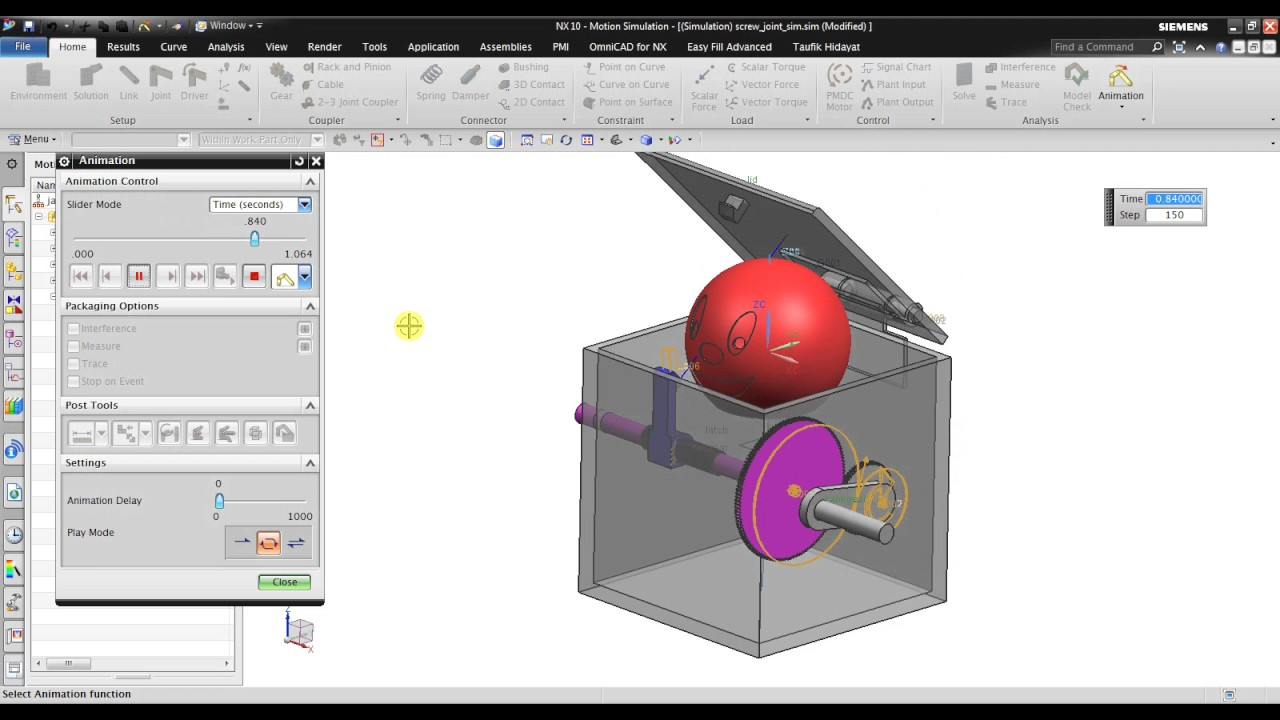
\includegraphics[height=6cm,width=1\textwidth,keepaspectratio]{motion_video2_preview.jpg}}
        % \caption{Click on a picture for a video}
        \label{fig:motion_video2_preview.jpg}
    \end{figure}
\end{frame}

\begin{frame}[t]{Motion Analysis}
    \framesubtitle{Task 1}
    \vspace{-0.6cm}
    \begin{figure}[H]
        \href{https://disk.yandex.ru/i/RsjuS-pJY70Oww}{
            \centering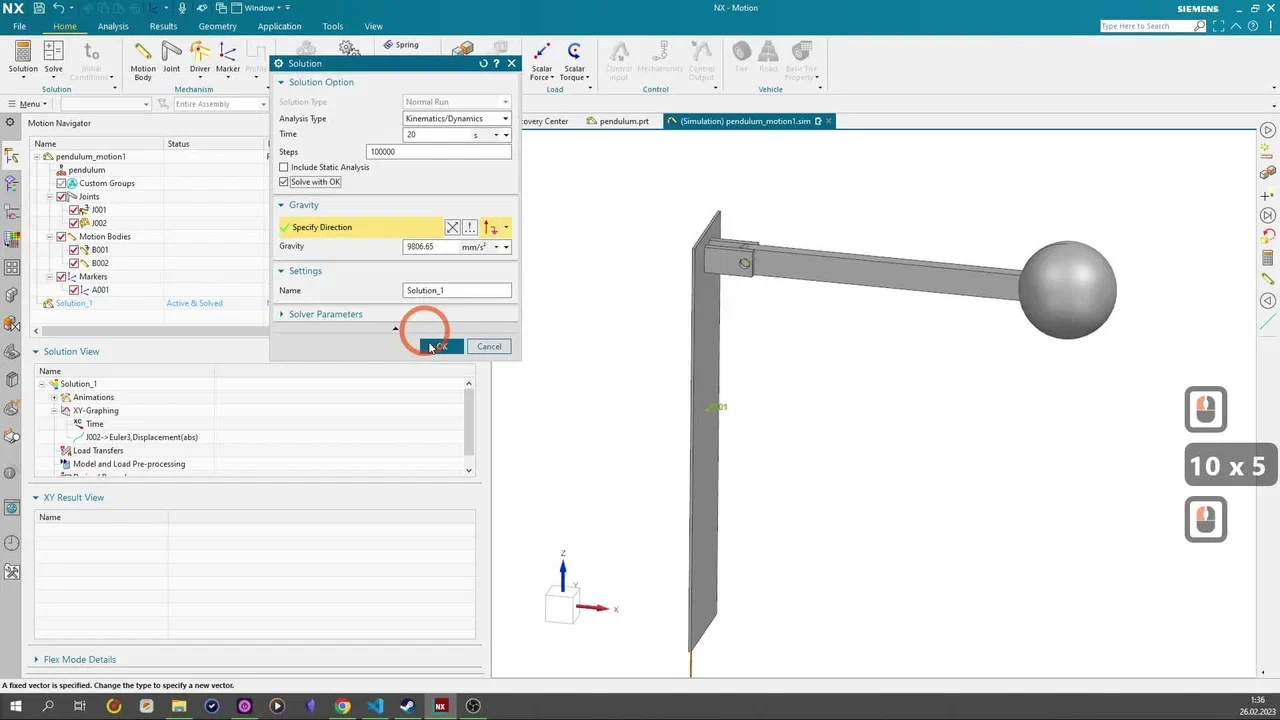
\includegraphics[height=6cm,width=1\textwidth,keepaspectratio]{motion_video_preview.png}}
        % \caption{Click on a picture for a video}
        \label{fig:motion_video_preview.png}
    \end{figure}
\end{frame}

\begin{frame}[t]{Reference Material}
\framesubtitle{}
\footnotesize
\begin{enumerate}
    \item \href{https://docs.sw.siemens.com/en-US/doc/209349590/PL20200605195244930.motion_designer/xid1334514}{Animation Designer documentation (official)}
    \item \href{https://docs.sw.siemens.com/en-US/doc/209349590/PL20200605195244930.mechatronics/id1101745}{Mechatronics Concept Designer documentation (official)}
    \item \href{https://docs.sw.siemens.com/en-US/doc/289054037/PL20201105153211099.motion/id563951}{Motion Simulation documentation (official)}
    \item \href{https://www.youtube.com/playlist?list=PLY2AphaX4SYcoXBPIjkHmph8JAtYcI90L}{Animation Designer Tutorials (video)}
    \item \href{https://www.youtube.com/playlist?list=PLY8N5WFx1MGAsxH7G49ey37QC_nFtQ72E}{NX Motion Simulation Tutorials (video)}
    \item \href{https://www.youtube.com/playlist?list=PLO4e9B3weuKLBmu6BEQkx3K7wE9GB_LL3}{Mechatronics Concept Designer (video)}
    \item \href{http://www2.me.rochester.edu/courses/ME204/nx_help/en_US/graphics/fileLibrary/nx/mechtronics/MCD_Quick_Start.pdf}{Mechatronics Concept Designer (book)}
    \item \href{https://www.clio-soft.ru/wp-content/uploads/2020/12/siemens-sw-simcenter-3d-solution-guide-e-book-russian.pdf}{All Simcenter 3D modules explanation (book, rus)}
    \item \href{https://www.ata-e.com/wp-content/uploads/2021/10/Siemens_Simcenter_3D_Solutions_Guide_e-Book_SET.pdf}{All Simcenter 3D modules explanation (book, eng)}
\end{enumerate}
    
\end{frame}

\fbckg{fibeamer/figs/last_page.png}
\frame[plain]{}

\end{document}